\documentclass[12pt]{article}
\usepackage[utf8]{inputenc}
\usepackage[a4paper,top=20mm]{geometry}
\usepackage{hyperref}
\usepackage{setspace}
\usepackage{amsfonts}
\usepackage{graphics}
\usepackage{tikz}
\graphicspath{ {./images/} }
\usepackage{graphicx}
\usepackage{amssymb}
\usepackage{amsmath}
\usepackage{parskip}
\newcommand\ddfrac[2]{\frac{\displaystyle #1}{\displaystyle #2}}
\newcommand*\circled[1]{\tikz[baseline=(char.base)]{
            \node[shape=circle,draw,inner sep=2pt] (char) {#1};}}
\DeclareMathOperator{\Deg}{deg}
\title{ZPC-24}
\author{Farhan, Raunak, Ishaan, Shreyas, Mudit}
\date{\today}
\doublespacing
\begin{document}

\maketitle
\title{\textbf{\underline{\fontsize{18}{12}\selectfont Instructions}}}\\
Please read the following instructions carefully before proceeding further:\\
\begin{enumerate}
\item The test is of 2 hours. It will end \textit{sharp} at \textbf{8:00 pm}.
\item Relevant reading material for all the questions has been provided in the document itself.
\item If you are stuck on a question that you cannot figure out, move on. Nothing good ever comes out of being hung up on something.
\item Please feel free to contact the invigilators in case of any queries.
\item We will provide hints to questions in the last hour, depending on the participation and responses.
\item All the best. GL HF :)\\
\end{enumerate}
\bigskip
\maketitle
\newpage
\title{\begin{center}\textbf{\underline{\fontsize{16}{12}\selectfont CAUCHY-SCHWARZ INEQUALITY}}\end{center}}

\section{Motivation For Cauchy-Schwarz Inequality}
Before starting with the inequality itself, we will try to figure out the geometric interpretation for the inequality. We know that the standard distance between two points in the 2-dimensional euclidean plane, say $x=(x_1,x_2)$ and $y=(y_1,y_2)$ is given by $$ d(x ,y)=\sqrt{(x_1-y_1)^2+(x_2-y_2)^2}$$
The above result can also be seen as a consequence of the Pythagorean theorem as shown in the figure below.
\begin{center}
    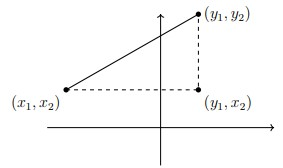
\includegraphics[]{images/zpc.jpg}
\end{center}
This standard distance also satisfies the triangle inequality, so, for any third point say $k$, we have $d(x,y)\leq d(x,k)+d(k,y)$. Putting $k$ as origin, we get: \\
$d(x.y)\leq d(x,0)+d(0,y)\Rightarrow \sqrt{(x_1-y_1)^2+(x_2-y_2)^2}\leq \sqrt{x_1^2+x_2^2}+\sqrt{y_1^2+y_2^2}$\\
$\Rightarrow x_1^2+y_1^2-2x_1y_1+x_2^2+y_2^2-2x_2y_2\leq x_1^2+x_2^2+y_1^2+y_2^2+2\sqrt{(x_1^2+x_2^2)(y_1^2+y_2^2)}$\\
Replace $y_1$ by $-y_1'$ and $y_2$ by $-y_2'$ to obtain:\\
$ \Rightarrow x_1^2+(-y_1')^2-2x_1(-y_1')+x_2^2+(-y_2')^2-2x_2(-y_2')\leq x_1^2+x_2^2+(-y_1')^2+(-y_2')^2+2\sqrt{(x_1^2+x_2^2)((-y_1')^2+(-y_2')^2)} $\\
$ \Rightarrow -2x_1(-y_1')-2x_2(-y_2')\leq 2\sqrt{(x_1^2+x_2^2)((-y_1')^2+(-y_2')^2)} $\\
$ \Rightarrow x_1y_1'+x_2y_2'\leq \sqrt{(x_1^2+x_2^2)(y_1'^2+y_2'^2)} \\ \Rightarrow (x_1^2+x_2^2)(y_1'^2+y_2'^2)\geq (x_1y_1'+x_2y_2')^2 $\\
The last statement is the Cauchy-Schwarz inequality for 2 variables in each set.

\section{The Cauchy-Schwarz Inequality}
\textbf{Theorem (Cauchy-Schwarz Inequality): }Let $(a_1, a_2,\dots , a_n)$ and $(b_l , b_2,\dots ,b_n)$ be
two sequences of real numbers, then we have:
$$ (a_1^2+a_2^2+\dots+a_n^2)(b_1^2+b_2^2+\dots+b_n^2)\geq (a_1b_1+a_2b_2+\dots+a_nb_n)^2$$
The equality holds, if and only if $(a_1, a_2,\dots , a_n)$ and $(b_l , b_2,\dots ,b_n)$ are proportional (which means that there exists a non-zero real number $k$ such that $a_i=kb_i$ for all $i=1,2,\dots,n$)\\
\underline{\textbf{Proof:}}\\
In this proof, we will use a quadratic function as follows:
$$ f(x)=(a_1x-b_1)^2+(a_2x-b_2)^2+\dots +(a_nx-b_n)^2$$
Note that $f(x)\geq0 $ always. Now, this is a quadratic function in $x$ which is always positive. So, if $D$ is the discriminant of this quadratic function then $D\leq 0$ (discriminant of $ax^2+bx+c$ is $D=b^2-4ac$). We can rewrite the above function as follows to obtain its discriminant:
$$f(x)=(a_1^2+a_2^2+\dots+a_n^2)x^2-2(a_1b_1+a_2b_2+\dots+a_nb_n)x+(b_1^2+b_2^2+\dots+b_n^2)$$
Now using the definition of discriminant and $D\leq0$, we get:
$$(a_1^2+a_2^2+\dots+a_n^2)(b_1^2+b_2^2+\dots+b_n^2)\geq (a_1b_1+a_2b_2+\dots+a_nb_n)^2$$
Also, note that for the equality to hold, $D=0$ which would imply that $a_ix-b_i=0\Rightarrow a_ix=b_i$ for all $i=1,2,\dots ,n$. So, the equality holds, if and only if $(a_1, a_2,\dots , a_n)$ and $(b_l , b_2,\dots ,b_n)$ are proportional.\\
\newpage
\section{Titu's Lemma}
In the theorem proved in the previous section, if we substitute $ \displaystyle a_i=\frac{x_i}{\sqrt{y_i}}$ and $ \displaystyle b_i=\sqrt{y_i}$, we get the following result:
$$\displaystyle\frac{x_1^2}{y_1}+\frac{x_2^2}{y_2}+\ldots+\frac{x_n^2}{y_n} \geq \frac{\left(x_1+x_2+\ldots+x_n\right)^2}{y_1+y_2+\ldots+y_n}$$
The above result is called as Titu's lemma and is very useful while solving problems.
\section{Some cool results}
In the Cauchy-Schwarz Inequality, if we take $b_i=1$ for all $i$, then we get the following:
$$\left(a_1+a_2+\ldots+a_n\right)^2 \leq n\left(a_1^2+a_2^2+\ldots+a_n^2\right)$$
Also, note that $\sqrt{a_1^2+b_1^2}+\sqrt{a_2^2+b_2^2} \geq \sqrt{\left(a_1+a_2\right)^2+\left(b_1+b_2\right)^2}$ from our initial triangle inequality argument. So, we have:
$$ \sqrt{a_1^2+b_1^2}+\sqrt{a_2^2+b_2^2}+\sqrt{a_3^2+b_3^2} \geq \sqrt{\left(a_1+a_2\right)^2+\left(b_1+b_2\right)^2}+\sqrt{a_3^2+b_3^2}$$ $$ \Rightarrow\sqrt{\left(a_1+a_2\right)^2+\left(b_1+b_2\right)^2}+\sqrt{a_3^2+b_3^2}\geq\sqrt{\left(a_1+a_2+a_3\right)^2+\left(b_1+b_2+b_3\right)^2}$$
Continuing the above process multiple times, we get :
$$\sqrt{a_1^2+b_1^2}+\sqrt{a_2^2+b_2^2}+\ldots+\sqrt{a_n^2+b_n^2} \geq \sqrt{\left(a_1+\ldots+a_n\right)^2+\left(b_1+\ldots+b_n\right)^2}$$


NOTE: Some problems might be more easy through the AM - GM inequality instead of the Cauchy-Schwarz Inequality. The AM-GM Inequality is that for $n$ positive real numbers $a_1,a_2,\dots,a_n$, we have $\displaystyle\frac{a_1+a_2+\ldots+a_n}{n} \geq \sqrt[n]{a_1 a_2 \ldots a_n}$
$$\square \square \square \square \square \square \square \square \square \square \square \square \square \square \square $$
\newpage
\maketitle
\title{\begin{center}\textbf{\underline{\fontsize{18}{12}\selectfont PROBLEMS}}\end{center}}
\begin{itemize}
    \item The questions here are all subjective, and will be graded on how well you can convince the checker of the mathematical rigour of your solution.
    \item The corresponding points of each question are mentioned with it. Do note that the points may or may not be proportionate to the relative difficulty of the question.
    \item The number of problems presented is much more than what is humanly possible to solve in the given time frame. Hence, prioritise correctness and rigour over number of problems solved.
    \item Note that any significant conclusion derived in the right direction to solve the problem may fetch you some points, so try to attempt all questions.
\end{itemize}
\bigskip
\bigskip
\bigskip
\begin{enumerate}
    \item Prove that for any positive real numbers $a,b$ and $c$,\\ $\left(\dfrac{a+b+c}{b+c}+\dfrac{a+b+c}{c+a}+\dfrac{a+b+c}{a+b}\right) \geq \dfrac{9}{2}.$ (1 point)\\
    \item Prove that for any positive real numbers $a,b$ and $c$,\\ $\left(\dfrac{a}{2a+b}+\dfrac{b}{2b+c}+\dfrac{c}{2c+a}\right) \leq 1$ (2 point)\\
    \item Let $a,b$ and $c$ be positive real numbers such that $abc = x, x\in (0,1]$. Prove that:\\
    $\left(\dfrac{1}{a^3(b+c)}+\dfrac{1}{b^3(c+a)}+\dfrac{1}{c^3(a+b)}\right) \geq \dfrac{3}{2}\sqrt[3]{x}$ (4 point)\\
    \item For positive real numbers $a,b,c$ and $d$, prove the following:\\
    $\left(\dfrac{a}{b^2+c^2+d^2}+\dfrac{b}{a^2+c^2+d^2}+\dfrac{c}{a^2+b^2+d^2}+\dfrac{d}{a^2+b^2+c^2}\right) \geq \dfrac{4}{a+b+c+d}$ (4 point)\\
    
    \item Let $a ,\ b,\ c$ be positive real numbers such that $a+b+c=1$, then prove that:\\
    $$\displaystyle\frac{a}{\sqrt{b+c}}+\frac{b}{\sqrt{c+a}}+\frac{c}{\sqrt{a+b}}\geq 
    \sqrt{\frac{3}{2}}$$ (5 points)\\
    
    \item Let $(n\geq 2)$ and let $I = \{1,2,3\cdots n-1,n\} $ and suppose  A = $\{A_i \mid i \in I\}$ and $B = \{B_i \mid i \in I\}$ be sets of mutually exclusive and collectively exhaustive events, with respect to a probability experiment. A set $S$ is said to contain mutually exclusive and collectively exhaustive, if:
    \begin{center}
    $\displaystyle\sum_{A \in S} P(A) = 1$ and $\forall x,y \in S \left(x \neq y \implies x \displaystyle \cap y = \phi\right)$
    \end{center}
    Prove that:
    $2\displaystyle\sum_{i<j}P(A_i)P(A_j) \leq \dfrac{n-2}{n-1} + \sum_{i=1}^{n}\frac{P(B_i)P(A_i)^2}{1-P(B_i)}$ (6 points)
\end{enumerate}
$$\square \square \square \square \square \square \square \square \square \square \square \square \square \square \square $$
\end{document}